%
% CRDT
%
Ein \gls{CRDT} ist eine spezielle Datenstruktur die in verteilten Systemen auf mehreren Geräten repliziert werden können. Jede Operation wird asynchron an alle Replikate gesendet. Jedes Replikat wendet alle ankommenden Aktualisierungen in variabler Reihenfolge an. Ein Algorithmus löst alle konfliktbehafteten Aktualisierungen auf, wodurch sichergestellt ist, dass Konflikte gar nicht erst auftreten~\cite{crdt_shapiro}. Eine Synchronisation ist nicht notwendig, da die Aktualisierung sofort ausgeführt wird ~\cite{crdt_shapiro2}.\\\\
%
In ihren Arbeiten betrachten Shapiro et. al zwei Replikationsmodelle in einem verteilten System: den zusandsbasierten und den operationsbasierten Ansatz.
Interessanterweise zeigen sie, dass diese beiden Replikationsmodelle und diese beiden Arten von CRDTs äquivalent sind.\\
Bei Operation-basierten \glspl{CRDT} muss sichergestellt werden, dass die Operationen nicht verloren gehen oder dupliziert werden wenn sie zu den anderen Replikaten übertragen werden.
Zustandsbasierte \glspl{CRDT} haben den Nachteil, dass der gesamte Zustand, statt nur der Operation, zu den anderen Replikaten übertragen werden muss.
%
%
\subsub{Zustandbasierter Ansatz}

\begin{figure}[H]
  \centering
  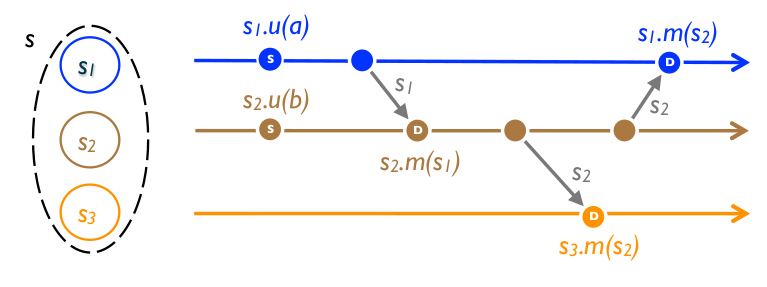
\includegraphics[width=0.8\textwidth]{crdt-state}
  \grayRule
  \caption[Replikation von zustandsbasierten \glspl{CRDT} Replikation]{Replikation von zustandsbasierten \glspl{CRDT}, Quelle: ~\cite{crdt_shapiro2}}
  \label{fig:crdt-state}
\end{figure}

Wenn ein Replikat ein Update von einem Client empfängt, aktualisiert es zuerst seinen lokalen Status und dann, einige Zeit später, seinen \b{vollständigen Status}.
So sendet jedes Replikat gelegentlich seinen vollständigen Status an ein anderes Replikat im System.
Um ein Replikat, das den Status eines anderen Replikats empfängt, wendet eine \b{Zusammenführungsfunktion} (merge) an, um den empfangenen Status mit dem lokalen Status zusammenzuführen.
Entsprechend sendet dieses Replikat gelegentlich auch seinen Status an ein anderes Replikat, sodass jedes Update schließlich alle Replikate im System erreicht.
%
%
\subsub{Operationsbasierter Ansatz}
\begin{figure}[H]
  \centering
  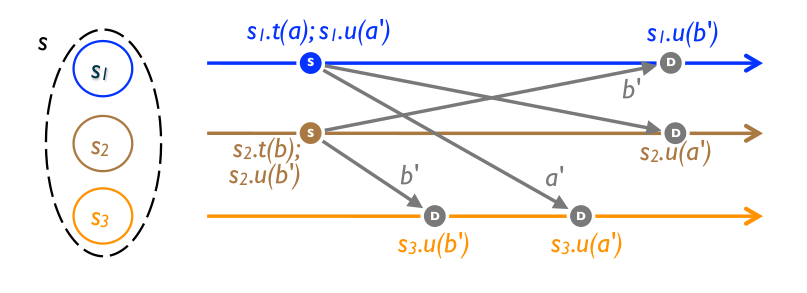
\includegraphics[width=0.8\textwidth]{crdt-op}
  \grayRule
  \caption[Replikation von Operationsbasierten \gls{CRDT}]{Replikation von Operationsbasierten \glspl{CRDT}, Quelle: ~\cite{crdt_shapiro2}}
  \label{fig:crdt-op}
\end{figure}

Bei diesem Ansatz sendet ein Replikat seinen vollständigen Status (kann groß sein) nicht an ein anderes Replikat.
Stattdessen sendet es nur den \b{Aktualisierungsvorgang} an \b{alle} anderen Replikate im System und erwartet von ihnen, dass sie das Update auf sich anwenden.\\
Da es sich um einen Sendevorgang handelt, wenn zwei Updates $u1$ und $u2$, bei einem Replikat $i$ angewendet werden und diese Updates an zwei Replikate $r1$ und $r2$ gesendet werden, können diese Updates in unterschiedlicher Reihenfolge bei diesen replikaten ankommen.
$r1$ kann sie in der Reihenfolge $u1, u2$ empfangen, während bei $r2$ die Updates in umgekehrter Reihenfolge ($u2, u1$) ankommen können.
Sind die Aktualisierungen \b{kommutativ}, können die Repliken zussamengeführt werden, egal in welcher Reihenfolge die Updates bei ihnen ankommen - der resultierende Zustand ist derselbe. In diesem Modell wird ein Objekt, für das alle gleichzeitigen Aktualisierungen kommutativ sind, CmRDT (commutative replicated data type - kommutativ replizierter Datentyp) genannt. \\\\
\b{Beispiel:...}\\
CRDTs befassen sich mit einem interessanten und grundlegendem Problem in verteilten Systemen, haben jedoch eine wichtige Einschränkung: "Da ein CRDT konstruktionsbedingt keinen Konsens verwendet, hat der Ansatz starke Einschränkungen; Dennoch sind einige interessante und nicht-triviale CRDTs bekannt" ~\cite{crdt_shapiro2}.
Die Einschränkung ist, dass die CRDT-Adresse nur einen Teil des Problemraums betrifft, da nicht alle möglichen Aktualisierungsoperationen kommutativ sind und daher nicht alle Probleme in CRDTs umgewandelt werden können. Auf der anderen Seite können CRDTs für einige Arten von Anwendungen durchaus nützlich sein, da sie eine nette Abstraktion zur Implementierung repliziter verteilter Systeme bieten und gleichzeitig theoretische Konsistenzgarantien bieten.
%
%Alas, everything in programming is trade-offs, so what do we trade for being able to have conflict-free data structures? Well, they are specialised data structures, like sets and counters, and not generic object representations like JSON, so we’ll have to buy into a whole world of these specialised data structures, and maybe we have hard time mapping our application objects to them. 